
The intital analysis for \bfive was done with $\texttt{robust = 0.5}$ (\bfiverobNS), same as the other three observing wavelengths. However, this caused some issues. 


Figure \ref{fig: Band5_robust05} shows the \SI and debiased polarized intensity maps, overplotted with the observed polarization vectors. Additionally, there are red vectors highlihgting the streamer, discussed in Chapter \ref{sec: streamer}. This is similar to Figure \ref{fig: StokesI_POLI_grid}. 




\textbf{Polarization Morphology:} When comparing the polarization morphology at the different \texttt{robust} values, 




\begin{figure}[htbp]
  \centering
  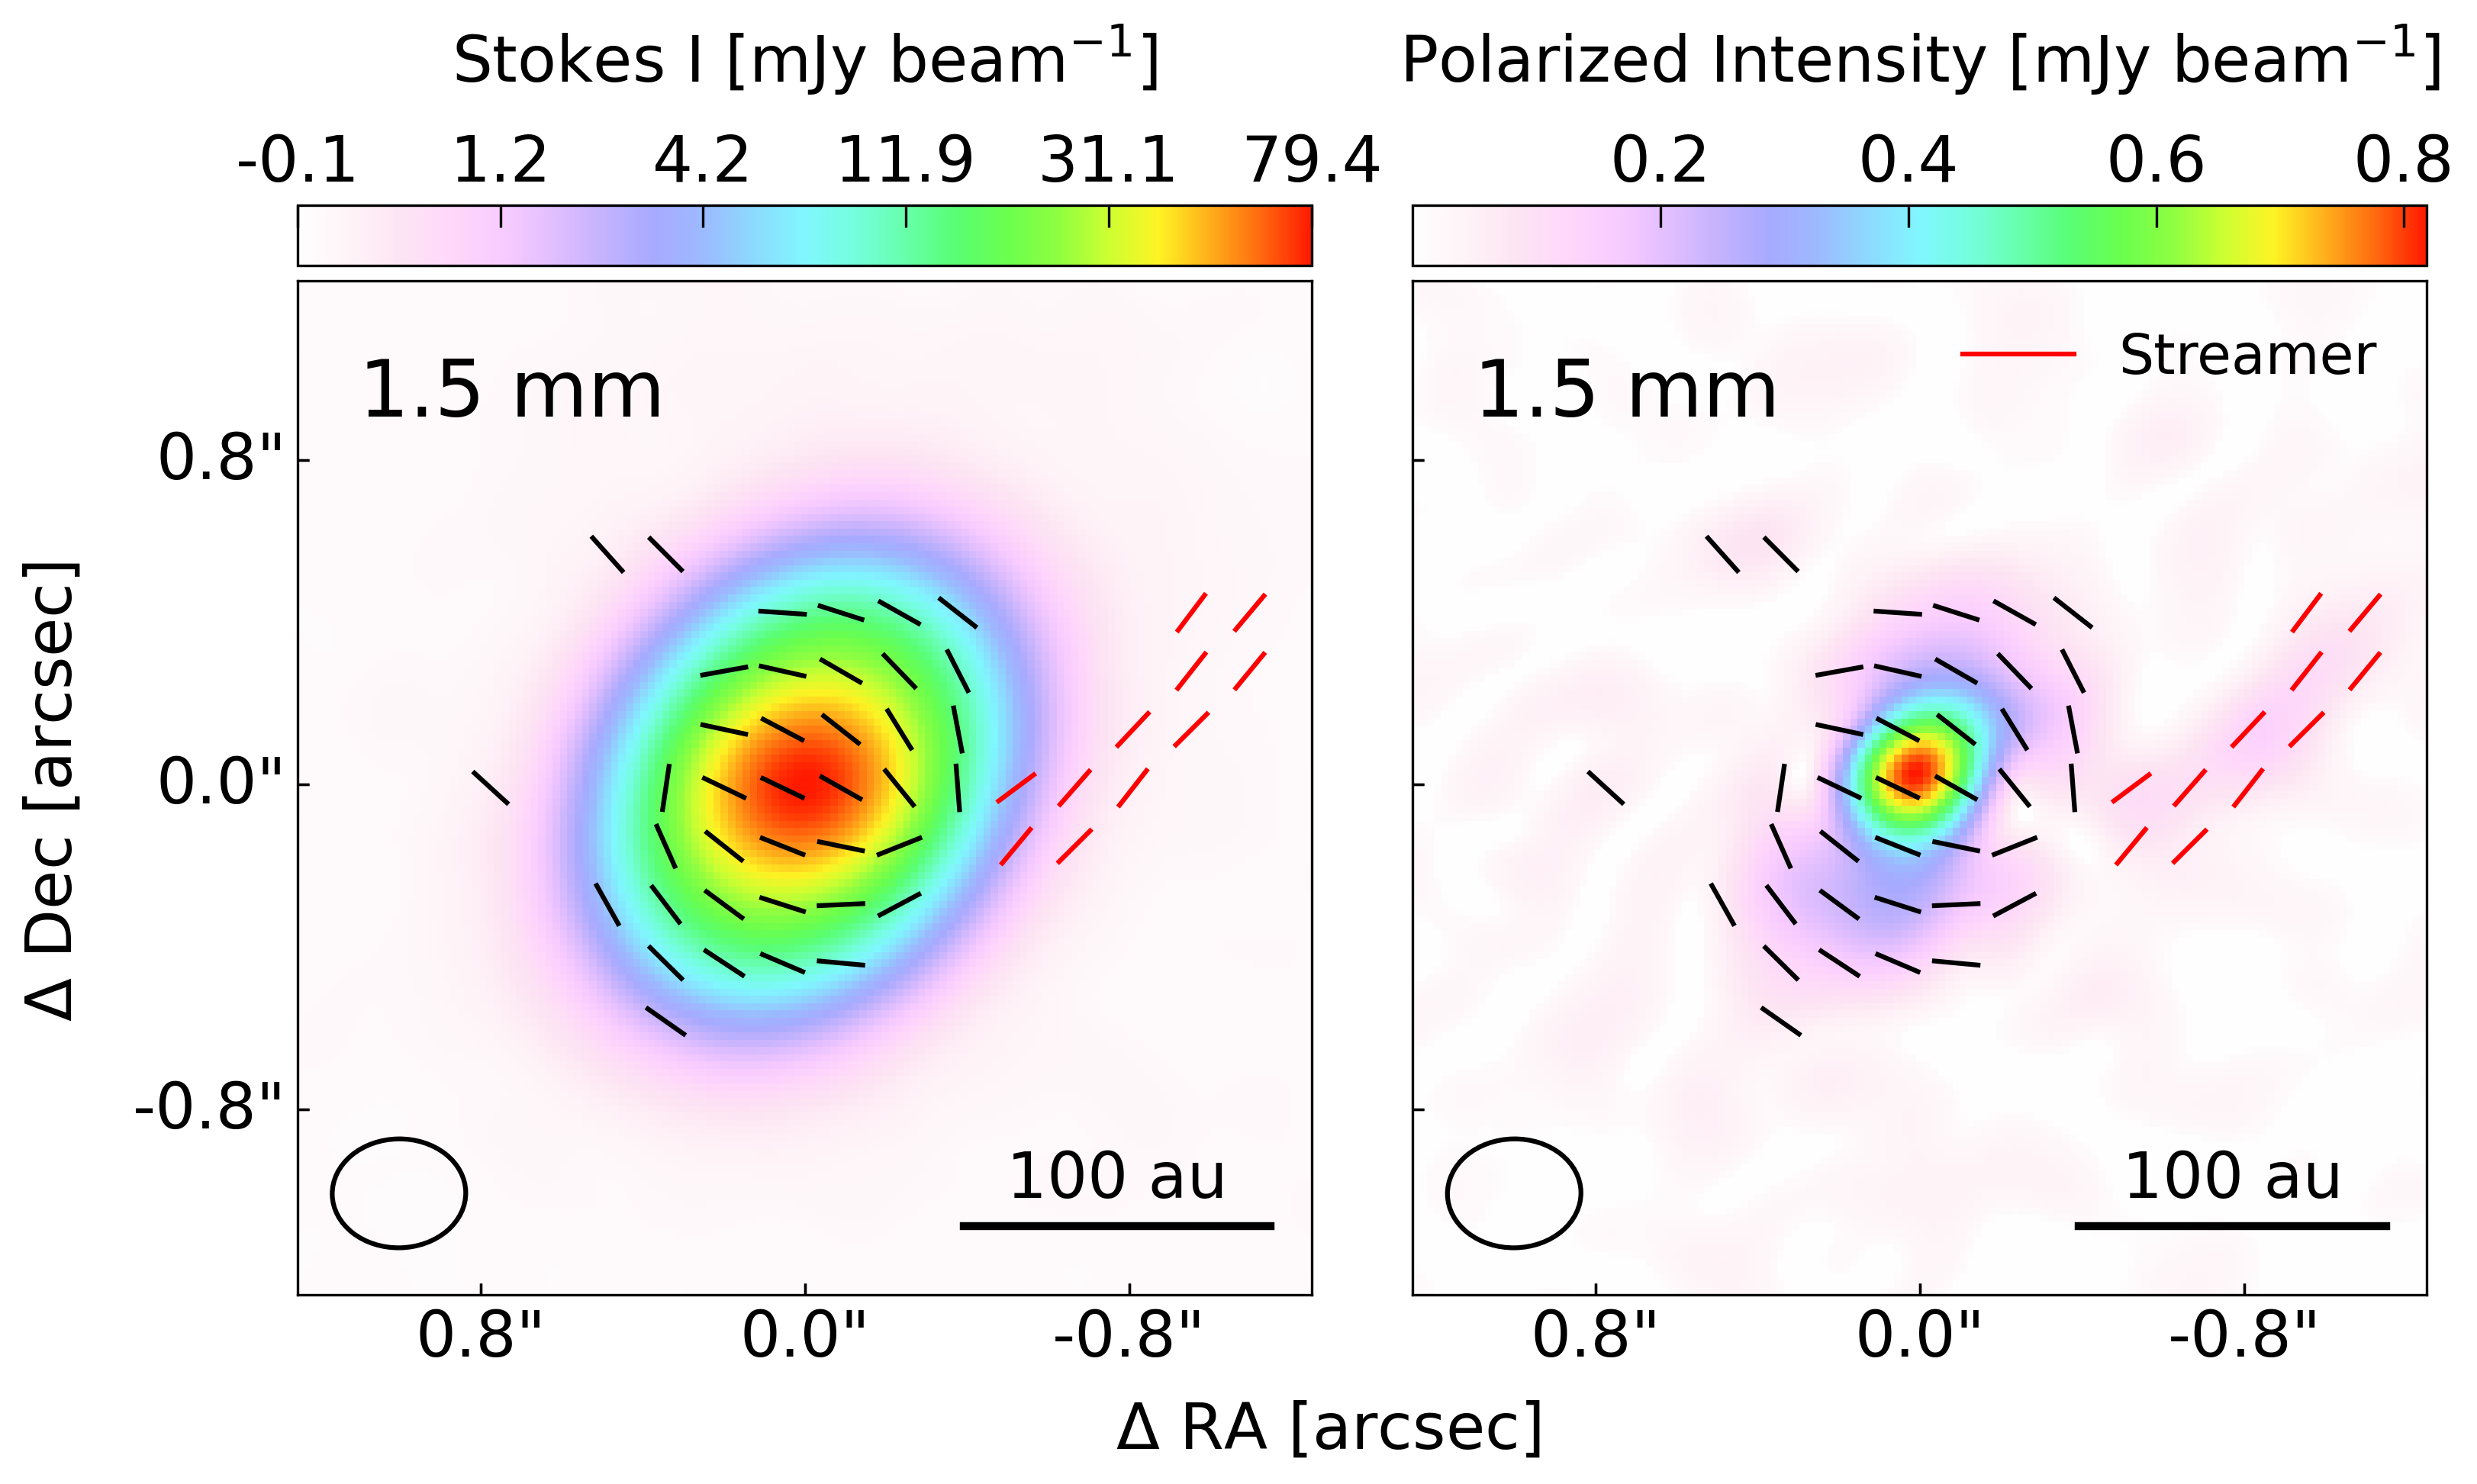
\includegraphics[width=0.99\textwidth]{WRITEUP_AND_IMAGES/IMAGES/WRITEUP/StokesI_POLI/IRS63_StokesI_POLI_vectors_BAND5_delta.png}
  \caption{Images of \SI (left) and debiased polarized intensity (right) for \bfive with \texttt{robust = 0.5}. The red vectors are for the streamer and are rotated by 90$^\circ$ to show magnetic field direction. Same plot as Figure \ref{fig: StokesI_POLI_grid}. \code{AU to au} }
  \label{fig: Band5_robust05}
\end{figure}